\documentclass[ignorenonframetext,]{beamer}
\setbeamertemplate{caption}[numbered]
\setbeamertemplate{caption label separator}{: }
\setbeamercolor{caption name}{fg=normal text.fg}
\beamertemplatenavigationsymbolsempty
\usepackage{lmodern}
\usepackage{amssymb,amsmath}
\usepackage{ifxetex,ifluatex}
\usepackage{fixltx2e} % provides \textsubscript
\ifnum 0\ifxetex 1\fi\ifluatex 1\fi=0 % if pdftex
\usepackage[T1]{fontenc}
\usepackage[utf8]{inputenc}
\else % if luatex or xelatex
\ifxetex
\usepackage{mathspec}
\else
\usepackage{fontspec}
\fi
\defaultfontfeatures{Ligatures=TeX,Scale=MatchLowercase}
\fi
\usetheme{Montpellier}
\usecolortheme{beaver}
% use upquote if available, for straight quotes in verbatim environments
\IfFileExists{upquote.sty}{\usepackage{upquote}}{}
% use microtype if available
\IfFileExists{microtype.sty}{%
\usepackage{microtype}
\UseMicrotypeSet[protrusion]{basicmath} % disable protrusion for tt fonts
}{}
\newif\ifbibliography

% Prevent slide breaks in the middle of a paragraph:
\widowpenalties 1 10000
\raggedbottom

\AtBeginPart{
\let\insertpartnumber\relax
\let\partname\relax
\frame{\partpage}
}
\AtBeginSection{
\ifbibliography
\else
\let\insertsectionnumber\relax
\let\sectionname\relax
\frame{\sectionpage}
\fi
}
\AtBeginSubsection{
\let\insertsubsectionnumber\relax
\let\subsectionname\relax
\frame{\subsectionpage}
}

\setlength{\parindent}{0pt}
\setlength{\parskip}{6pt plus 2pt minus 1pt}
\setlength{\emergencystretch}{3em}  % prevent overfull lines
\providecommand{\tightlist}{%
\setlength{\itemsep}{0pt}\setlength{\parskip}{0pt}}
\setcounter{secnumdepth}{0}
\usepackage[retainorgcmds]{IEEEtrantools}

\title{Conditional Quantile Regression Article Proposal}
\author{Marcelo Ruas}
\date{Sep 29, 2017}

\begin{document}
\frame{\titlepage}

\begin{frame}{Overview}

\begin{itemize}
\item
  Let a time series be given by
  \[y_t = A(L)y_t + \beta x_t + \varepsilon_t,\] where the distribution
  of \(\varepsilon_t\) is unknown. In this case, the usage of a
  parametric model is hardly atrrative.
\item
  Quantile regression is one technique available to model this time
  series dynamics, by estimating a phin grid of \(\alpha\)-quantiles at
  once and forming a data-driven conditional distribution.
\item
  We explore different strategies of estimating the Conditional Quantile
  Regression focused on approaching the conditional distribution or
  \(y_{t+h|t}\), for a given horizon \(h\).
\end{itemize}

\end{frame}

\section{Linear Models}\label{linear-models}

\begin{frame}{Linear Models - Formulation}

\begin{IEEEeqnarray}{lr}
	\min_{\beta_{0\alpha},\beta_\alpha,\varepsilon_{t\alpha}^{+}, \varepsilon_{t\alpha}^{-}} \, \sum_{\alpha \in A} \sum_{t \in T}\left(\alpha \varepsilon_{t \alpha}^{+}+(1-\alpha)\varepsilon_{t \alpha}^{-}\right) \span \label{eq:linear-opt-1}\\
	\mbox{subject to} \span \nonumber \\
	\varepsilon_{t \alpha}^{+}-\varepsilon_{t \alpha}^{-}=y_{t} - \beta_{0\alpha} - \beta_{\alpha}^T x_{t}, & \forall t \in T,\qquad \forall \alpha \in A, \\
	\varepsilon_{t\alpha}^+,\varepsilon_{t\alpha}^- \geq 0, &  \forall t \in T,\forall \alpha \in A,\\ 
	\beta_{0\alpha} + \beta_{\alpha}^T x_{t} \leq \beta_{0\alpha'} + \beta_{\alpha'}^T x_{t}, \span \nonumber \\
	\span \label{eq:linear-opt-ult} \forall t \in T, \forall (\alpha, \alpha') \in A \times A,  \alpha < \alpha',
\end{IEEEeqnarray}

\end{frame}






\begin{frame}{Linear Models - Resume}

\begin{itemize}
\item
  As there are many explanatory variables for \(y_t\), it is interesting
  to do a regularization process in order to select only a subset to
  compose the model.
\item
  The next slides are going to cover a few different ways to achieve
  this using Mixed Integer Linear Programming.
\end{itemize}

\end{frame}


\begin{frame}{Regularization by MILP - Resume}

\begin{itemize}
\item
  MILP models allow only \(K\) variables to be used for each
  \(\alpha\)-quantile. This means that only \(K\) coefficients
  \(\beta_{p\alpha}\) may have nonzero values, for each
  \(\alpha\)-quantile. It must be guaranteed by constraints on the
  optimization problem.
\item
  We present three forms of grouping probabilities while selecting
  variables
\end{itemize}

\end{frame}

\begin{frame}{One model for each \(\alpha\)-quantile - Formulation}

\tiny

%\begin{eqnarray}
% \underset{\beta_{0\alpha},\beta_\alpha,z_{p \alpha} \varepsilon_{t \alpha}^{+},\varepsilon_{t \alpha}^{-}}{\text{min}} & \sum_{\alpha \in A} \sum_{t\in T}\left(\alpha\varepsilon_{t \alpha}^{+}+(1-\alpha)\varepsilon_{t\alpha}^{-}\right) \label{eq:mip0} \\
%\mbox{s.t } & \varepsilon_{t \alpha}^{+}-\varepsilon_{t \alpha}^{-}=y_{t}-\beta_{0 \alpha}-\sum_{p=1}^{P}\beta_{p \alpha}x_{t,p},& \qquad\forall t \in T ,\forall \alpha \in A, \label{eq:mip1}\\
%& \varepsilon_{t \alpha}^{+},\varepsilon_{t \alpha}^{-}\geq0,&\qquad\forall t \in T ,\forall \alpha \in A, \label{eq:mip2}\\
%& - M z_{p \alpha} \leq \beta_{p \alpha} \leq M z_{p \alpha},&\qquad \forall \alpha \in A, \forall p\in P, \label{eq:mip3}\\
%& \sum_{p=1}^P z_{p \alpha} \leq K, & \qquad \forall \alpha \in A, \label{eq:mip4}\\
%& z_{p \alpha} \in \{0,1\},&\qquad \forall \alpha \in A, \forall p\in P, \label{eq:mip5}\\
%& \beta_{0\alpha} + \beta_{\alpha}^T x_{t} \leq \beta_{0\alpha'} + \beta_{\alpha'}^T x_{t}, & \qquad \forall t \in T, \forall (\alpha, \alpha') \in A \times A,  \alpha < \alpha',\nonumber\\ \label{eq:mip6}
%\end{eqnarray}

\begin{IEEEeqnarray}{lr}
	\underset{\beta_{0\alpha},\beta_\alpha,z_{p \alpha}, \varepsilon_{t \alpha}^{+},\varepsilon_{t \alpha}^{-}}{\text{min}} \sum_{\alpha \in A} \sum_{t\in T}\left(\alpha\varepsilon_{t \alpha}^{+}+(1-\alpha)\varepsilon_{t\alpha}^{-}\right) \span \label{eq:mip0}  \\
	\mbox{subject to} \span \nonumber \\
	\varepsilon_{t \alpha}^{+}-\varepsilon_{t \alpha}^{-}=y_{t}-\beta_{0 \alpha}-\sum_{p=1}^{P}\beta_{p \alpha}x_{t,p}, \span \nonumber  \\
	& \forall t \in T ,\forall \alpha \in A, \label{eq:mip1}  \\
	\varepsilon_{t \alpha}^{+},\varepsilon_{t \alpha}^{-}\geq0, & \forall t \in T ,\forall \alpha \in A, \label{eq:mip2}\\
	- M z_{p \alpha} \leq \beta_{p \alpha} \leq M z_{p \alpha}, & \forall \alpha \in A, \forall p\in P, \label{eq:mip3}\\
	\sum_{p=1}^P z_{p \alpha} \leq K, & \forall \alpha \in A, \label{eq:mip4}\\
	z_{p \alpha} \in \{0,1\}, & \forall \alpha \in A,  \forall p\in P, \label{eq:mip5}\\
	\beta_{0\alpha} + \beta_{\alpha}^T x_{t} \leq \beta_{0\alpha'} + \beta_{\alpha'}^T x_{t},  \nonumber \\
	\quad \qquad \qquad \forall t \in T, \forall (\alpha, \alpha') \in A \times A,  \alpha < \alpha', \span \label{eq:mip6}
\end{IEEEeqnarray}


\end{frame}

\begin{frame}{Defining groups for \(\alpha\)-quantiles - Formulation}

\tiny

\begin{eqnarray}
 \underset{\beta_{0\alpha},\beta_\alpha,z_{p \alpha} \varepsilon_{t \alpha}^{+},\varepsilon_{t \alpha}^{-}}{\text{min}} & \sum_{\alpha \in A} \sum_{t\in T}\left(\alpha\varepsilon_{t \alpha}^{+}+(1-\alpha)\varepsilon_{t\alpha}^{-}\right) \label{eq:mip0} \\
\mbox{s.t } & \varepsilon_{t \alpha}^{+}-\varepsilon_{t \alpha}^{-}=y_{t}-\beta_{0 \alpha}-\sum_{p=1}^{P}\beta_{p \alpha}x_{t,p},& \qquad\forall t \in T ,\forall \alpha \in A, \label{eq:mip1}\\
& \varepsilon_{t \alpha}^{+},\varepsilon_{t \alpha}^{-}\geq0,&\qquad\forall t \in T ,\forall \alpha \in A, \label{eq:mip2}\\
& - M z_{p \alpha g} \leq \beta_{p \alpha} \leq M z_{p \alpha g},&\qquad \forall \alpha \in A, \forall p\in P, \forall g \in G \label{eq:mip3}\\
&z_{p \alpha g} := 2 - ( 1-z_{pg}) - I_{g\alpha}& \label{mipgrupzpa} \\
& \sum_{p=1}^P z_{p g} \leq K, & \qquad \forall g \in G, \label{eq:mip4}\\
& \beta_{0\alpha} + \beta_{\alpha}^T x_{t} \leq \beta_{0\alpha'} + \beta_{\alpha'}^T x_{t}, & \qquad \forall t \in T, \forall (\alpha, \alpha') \in A \times A,  \alpha < \alpha',\nonumber\\ \label{eq:mip6} \\
& \sum\limits_{g \in G} I_{g\alpha} = 1, & \forall \alpha \in A,\label{eq:mipgrupa} \\
& I_{g\alpha}, z_{pg} \in \{0,1\},& \forall p \in P, \quad \forall g \in G, 
\end{eqnarray}

\end{frame}

\begin{frame}{Defining groups by the introduction of switching variable
- Formulation}

\tiny

\begin{eqnarray}
\underset{\beta_{0\alpha},\beta_\alpha,z_{p \alpha} \varepsilon_{t \alpha}^{+},\varepsilon_{t \alpha}^{-}}{\text{min}} & \sum_{\alpha \in A} \sum_{t\in T}\left(\alpha\varepsilon_{t \alpha}^{+}+(1-\alpha)\varepsilon_{t\alpha}^{-}\right) \label{eq:mipgr0} \\
\mbox{s.t } & \varepsilon_{t \alpha}^{+}-\varepsilon_{t \alpha}^{-}=y_{t}-\beta_{0 \alpha}-\sum_{p=1}^{P}\beta_{p \alpha}x_{t,p},& \qquad\forall t \in T ,\forall \alpha \in A, \label{eq:mipgr1}\\
& \varepsilon_{t \alpha}^{+},\varepsilon_{t \alpha}^{-}\geq0,&\qquad\forall t \in T ,\forall \alpha \in A, \label{eq:mipgr2}\\
& - M z_{p \alpha} \leq \beta_{p \alpha} \leq M z_{p \alpha},&\qquad \forall \alpha \in A, \forall p\in\{1,\dots,P\}, \label{eq:mipgr3}\\
& \sum_{p=1}^P z_{p \alpha} \leq K, & \qquad \forall \alpha \in A, \label{eq:mipgr4}\\
& z_{p \alpha} \in \{0,1\},&\qquad \forall \alpha \in A, \forall p\in\{1,\dots,P\}, \label{eq:mipgr5}\\
& \beta_{0\alpha} + \beta_{\alpha}^T x_{t} \leq \beta_{0\alpha'} + \beta_{\alpha'}^T x_{t}, & \qquad \forall t \in T, \forall (\alpha, \alpha') \in A \times A,  \alpha < \alpha',\nonumber\\ \label{eq:mipgr6} \\
& z_{p\alpha} - z_{p\alpha+1} \leq m_{p\alpha}, & \qquad \forall \alpha \in A', \qquad \forall p \in P  \\
& \sum_{\alpha \in A'} r_\alpha \leq |G| - 1 
\label{eq:mipgr} \\
\end{eqnarray}

where \(A' = A\setminus \{|A|\}\) \normalsize

\end{frame}

\section{Nonparametric model}\label{nonparametric-model}

\begin{frame}{Nonparametric model - Formulation}

\tiny

\begin{eqnarray}
\min_{q_{\alpha t},\delta^+_{t}, \delta_t^-, \xi_t} & \sum_{\alpha \in A} \sum_{t \in T'}\left(\alpha\delta_{t \alpha }^{+}+(1-\alpha)\delta_{t \alpha }^{-}\right) & \\
& \qquad \qquad \qquad \qquad \qquad + \lambda_1\sum_{t \in T'}\gamma_{t \alpha } + \lambda_2\sum_{t \in T'}\xi_{t \alpha } & \nonumber \\
s.t. & \delta_{t}^{+}-\delta_{t \alpha }^{-}=y_{t}-q_{t \alpha }, & \qquad\forall t \in T',\forall \alpha \in A,\\
   & D^{1}_{t \alpha }=\frac{q_{\alpha t+1}-q_{\alpha t}}{x_{t+1}-x_{t}},
    & \qquad\forall t \in T',\forall \alpha \in A,\\   
 & D^{2}_{t \alpha }=\frac{\left(\frac{q_{\alpha t+1}-q_{\alpha t}}{x_{t+1}-x_{t}}\right)-\left(\frac{q_{\alpha t}-q_{\alpha t-1}}{x_{t}-x_{t-1}}\right)}{x_{t+1}-2x_{t} + x_{t-1}}.
  & \qquad\forall t \in T',\forall \alpha \in A,\\
 & \gamma_{t \alpha}\geq D^1_{t \alpha }, & \qquad\forall t \in T',\forall \alpha \in A,\\
  & \gamma_{t \alpha}\geq-D^1_{t \alpha}, & \qquad\forall t \in T',\forall \alpha \in A,\\
  & \xi_{t \alpha}\geq D^2_{t \alpha }, & \qquad\forall t \in T',\forall \alpha \in A,\\
 & \xi_{t \alpha}\geq-D^2_{t \alpha}, & \qquad\forall t \in T',\forall \alpha \in A,\\
 & \delta_{t \alpha}^{+},\delta_{t \alpha}^{-},\gamma_{t \alpha}, \xi_{t \alpha}\geq0, & \qquad\forall t \in T',\forall \alpha \in A,\\
  & q_{t \alpha} \leq q_{t \alpha'}, & \qquad \forall t \in T', \forall (\alpha, \alpha') \in A \times A, \alpha < \alpha',\nonumber \\  
  \end{eqnarray}

\end{frame}

\begin{frame}{Nonparametric vs.~Linear Model}

\begin{itemize}
\tightlist
\item
  The nonparametric approach is more flexible to capture
  heteroscedasticity.
\end{itemize}

\begin{figure}
  \centering
  \begin{minipage}[t]{\linewidth}
    \centering
    \begin{minipage}[t]{0.45\linewidth}
      \centering     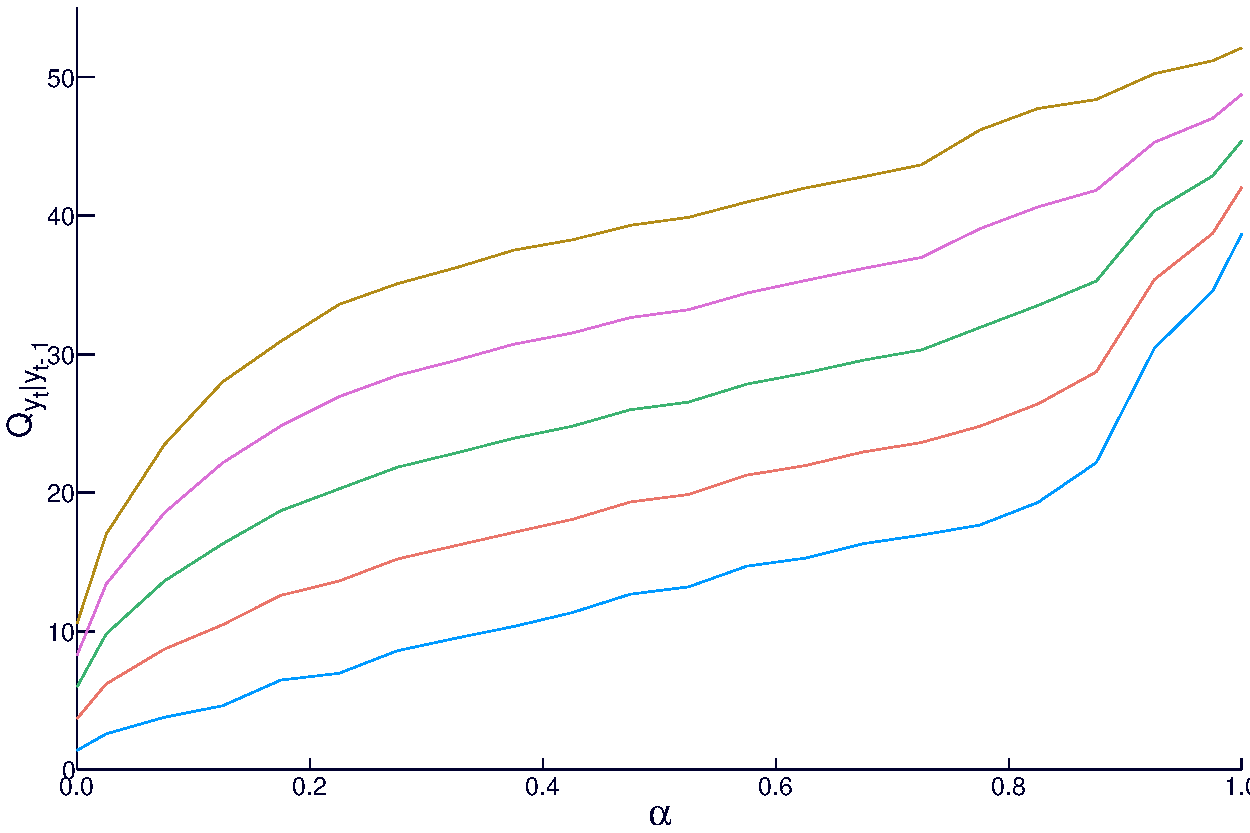
\includegraphics[width=\textwidth]{../Figuras/regressao-quantilica/icaraizinho-quantile-linear}
    \end{minipage}
    \begin{minipage}[t]{0.45\linewidth}
      \centering     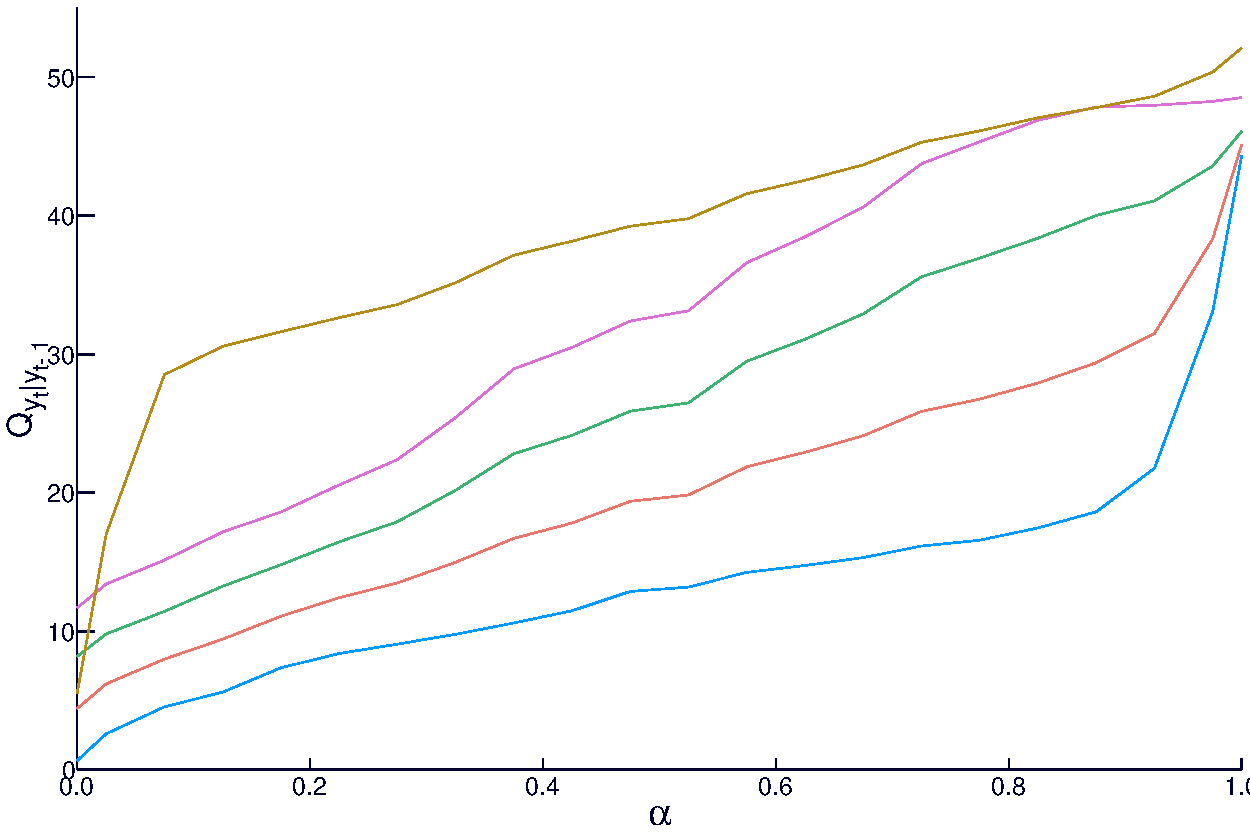
\includegraphics[width=\textwidth]{../Figuras/regressao-quantilica/icaraizinho-quantile-nonpar-lambda30}
    \end{minipage}
  \end{minipage}
  \caption{Estimated quantile functions, for different values of $y_{t-1}$. On the left using a linear model and using a nonparametric approach on the right.}
  \label{fig:quantiles-vs-xt}
\end{figure}

\end{frame}

\begin{frame}{Nonparametric vs.~Linear Model}

\begin{itemize}
\tightlist
\item
  This flexibility might lead to overfitting, if we don't select a
  proper penalty, as shown below:

  \begin{figure}
          \centering     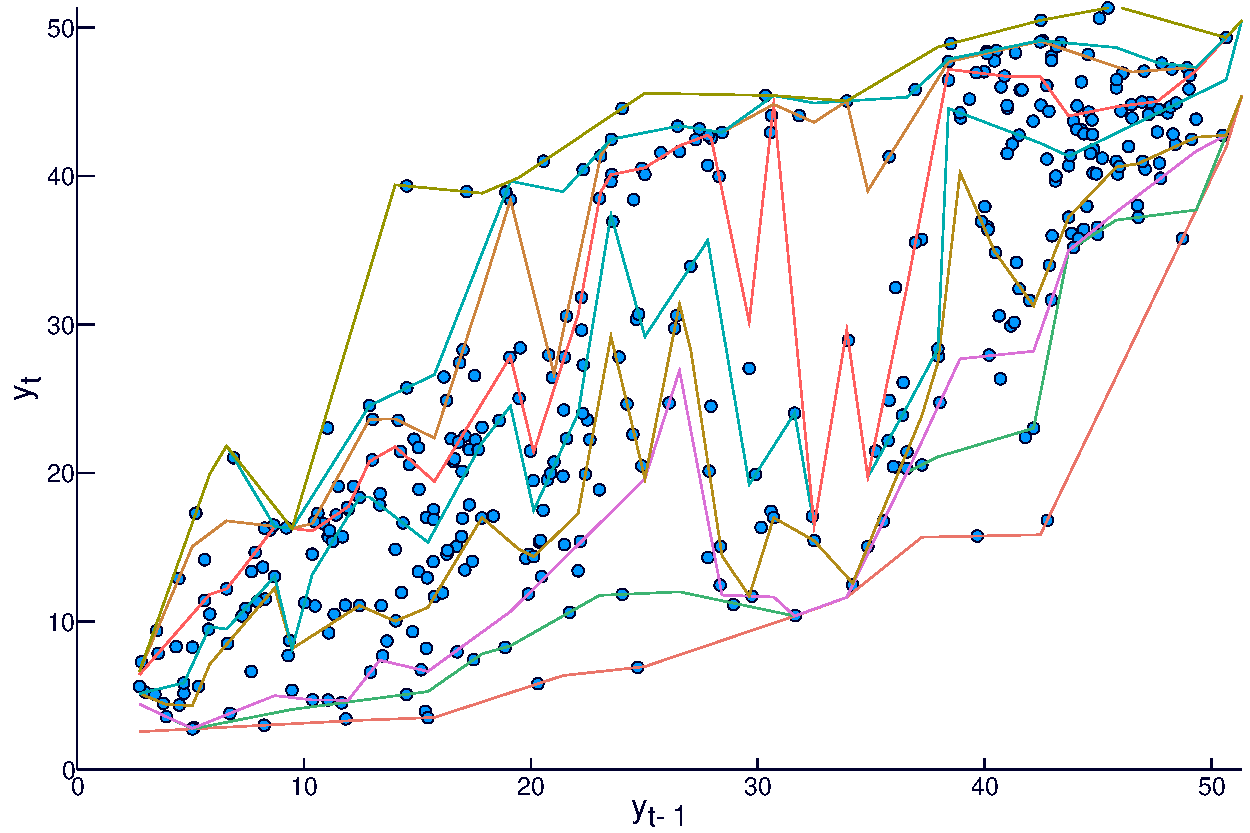
\includegraphics[width=0.6 \textwidth]{../Figuras/regressao-quantilica/icaraizinho-crossing-01}
  \caption{Example of a overfitted quantile function}
  \label{fig:convergence}
  \end{figure}
\end{itemize}

\end{frame}

\section{Goals}\label{goals}

\begin{frame}{Goals}

Goals of this work are:

\begin{itemize}
\item
  Using multiple quantiles to estimate the empirical conditional
  distribution of variables in a time series
\item
  Producing a model identification methodology
\item
  Natural Ressources and Financial applications
\end{itemize}

\end{frame}

\end{document}
